%!TEX root = project.tex

\chapter*{About this project}
\paragraph{Abstract}

This project was contracted to us through Enterprise Ireland1[1] from a company called RoamPA. We have previously worked on a project for RoamPA in the past. RoamPA was building a web application aimed at business users and required two modules to be developed for them externally. One of the modules consists of generating reports for a user based on streamlined, friendly queries for user in a management position. This system would let the user generate queries about users or groups of users relating to their business activities. The other module consists of a reviews system which allows users to generate reviews about businesses,faculties, points of interest etc. The review system requires the ability to create, view, like and dislike reviews, all of which is presented to the user through a map. Both of these modules had to be created from scratch and had to integrate into their existing server environment whilst using their database technologies. There was a lot of requirements, frameworks and dependencies. This project was a great experience and because it required knowledge about technologies we had never used before so we were delighted to take this challenge.

\paragraph{Authors}

The authors of this project are Andrew Sweeney and John Frizzell. We are both graduates of the BSc in Computing in Software Development which was the preceding course to the current honours degree. We both have a great interest in programming and technology. We are constantly seeking ways to improve our knowledge and skills.


\chapter{Introduction}

RoamPA Ltd is a start-up company founded by Una McNeill. They are developing a web application which is used to streamline the process of moving employees globally for work and business purposes. They wish to provide a much improved employee experience, significant cost savings to clients and greater return on investments with assignments and business travel.

We had previously worked for her on another project. The previous project had brought us outside the scope of our college work and proved to be a great learning experience. A year later We were asked again if they would develop two separate modules for this web application.

This time the focus of the project was completely different. This new project involved technologies and methodologies new to us. The focus was to create a reviews system where a user can view, create and rate reviews. The reviews would be then displayed an some form of map.\newline

\textbf{JOHNS BIT ABOUT REPORT GENERATOR}\newline

All of these technologies were outside of the scope of our college work and required a lot of research, experimentation and tutorials to complete the solution. Aside from programming in Java through our coursework and having some experience with MySQL databases we hadn't any previous experience with these technologies. Our course work covered some basic HTML and CSS in first year, so all of the skills to develop this application were learned as we went and through other experiences with web technologies.


\chapter{Context}

\section{Why we chose this project}

Throughout our college course we have developed in many different languages. Java, C\#, C and Python to name a few. We have not had the chance to really to dig deeply into web development. Web languages like PHP and Javascript were not part of our syllabus. Our sister course "Computing in Digital Media" does some of the design elements of web development but not much of the back-end stuff that we've both liked. Throughout our course we had a few semesters that had Database modules involving MYSQL. We heard the current project involved full blown MVC, Servlets, ORM and JSP pages. We also learned that the main language required for the project was Java which is one of the core languages for our college course. This project gave us a whole new area to experiment with and learn. Due to the challenge and interest we accepted the contract for this project.

\section{Challenges we had to face}    

Straight from the beginning, the challenge was to understand all of the frameworks and how all of the different parts of the environment work together. This meant completely understanding concepts like ORM and how they are applied through the framework Hibernate. Other concepts included learning how MVC is applied through SpringMVC with routes etc. There was a lot to research, a lot of frameworks to read up on. There was also numerous dependencies to figure out and all of this had to be. The amount of research, tutorials and understanding to be put into the project was the challenge. 


\section{Objectives}

\begin{itemize}
\item{Follow the specifications provided to make integration easier}
\item{Research the frameworks and environment}
\item{Create a reports module}
\item{Create a reviews module}
\end{itemize}

\section{Specifications}

We were creating a two modules for RoamPA. Both modules had to be integrated onto RoamPA's existing Apache Tomcat server. The Frameworks required of us were to use Hibernate ORM and SpringMVC. The existing database RoamPA uses is MySQL. All of the code handed over to RoamPA must be integrable on their server.

The first module involved creating a reviews system. The reviews system should allow the customer to look up an area using a search box and using filters then find locations for buildings like hospitals,restaurants and numerous other points of interest. The customer could then click on the POI and create a review for a business. They can also rate a current review that exists on there and like or dislike it.

The second module \newline

\textbf{JOHNS BIT ABOUT REPORT GENERATOR}


\chapter{Methodology}

Consisting of a team of two we communicated weekly through Skype calls,reviewing over each others code. The process was incremental as we first primarily spending a lot of time researching and understanding the environment. We went through cycles of researching and going through tutorials on Hibernate and then later on tutorials for SpringMVC. This helped reinforce our understanding of how everything worked. At times we would meet up to do some paired programming, this proved as a great experience as we were able to help each other understanding the project a lot quicker. The was numerous cycles of experimenting with Hibernate, trying pass information through it to the database and gradually building up knowledge from there. 

We used GitHub as a repository for our code. This is how the code you later be passed over to the developers at RoamPA. Using GitHub enabled us to download each others work and test locally. GitHub greatly helped our work-flow enabling us to share code between us in minutes remotely from home.

We were restrained to using technologies that would only work on an Apache Tomcat server. This means programming using the following

\begin{itemize}
	\item{Programming all of the server backend in Java}
	\item{Designing all of the webpages using HTML/CSS Javascript and JQuery, these then were later fitted into JSP pages}
	\item{Keeping all of the database queries to conform with MySQL}
	\item{Using Hibernate to facilitate the passage of data too and from the database}
	\item{Using SpringMVC to manage the structure of the project}
\end{itemize}

This meant the only real choice in technologies to use we had was deciding on what map API to use.

Google Maps was always the first consideration for what mapping API would use. The most well known and popular choice may not always be the best solution to the problem. This lead us to experimenting with several other map API's. Alternatives involved looking at Bing Maps, OpenStreetMap and Leaflet. Even with all of the choice Google Maps still proved to be the best selection. There were varying reasons for not using tha alternatives primarily because of terms of contract, the cost and the map API's being relatively new left them open to change in future. Google Maps has been around 11 years and is constantly updated. Google Maps API allowed querying exactly what we wanted. Google Places is part of the Google Maps API and allows for querying using different type filters. An example of some of the type filters are airports,libraries, department stores, restaurants etc. You can pass in a location, a filter and a radius to the API and have all businesses of that type returned back in JSON format. \newline

\section{Introduction}
In the context of the time span of computing, Word of Mouth (WOM) has long been shown to be efficacious and an important source of information when consumers wish to make purchasing decisions\cite{Nielsen}. The usage of Word of Mouth as a marketing tool dates back to, at least, the 1970s, after psychologist George Silverman created his 'Word of Mouth Model' after observing focus groups of physicians disucssing pharaceutical products~\cite{WOM}. Here he found that within a focus group the positive opinion of one physician could sway other members of the group who had previously been skeptical, and even the opinions of those whose patients had had negative experiences with a particular drug.

With the rapid proliferation of digital services that allow consumers to review services online this model is now applied as an Electronic Word of Mouth (eWOM), in 2008 Nielsen Online found that 81\% of online shoppers read online reviews from other customers and 71\% agreed that these reviews made them more comfortable in purchasing the product, in comparison only 14\% sought out reviews from an established source~\cite{Nielsen}. In the case of tourism B. Brown of the University of Glasgow concluded that tourists will use online reviews as a way to "pre-visit" locations~\cite{Brown}.

Many sites and web platforms supply the user with the ability review services or goods, hoever, the quality and quantity of these reviews vary greatly~\cite{Zhang}.

\section{Body}
We know that in the field of traditional marketing, by 'Word of Mouth', that the perceived expertise of the reviewer correlates to how likely it is that the receiver will pay attention to the information on offer~\cite{Bansal}. Given that most reviews online are anonymous or tied to identities which the receiver of the review knows nothing about this perceived expertise must be attained in other ways:

Lopez et al\cite{Lopez} performed research on the \emph{yelp.com} platform comparing the 'usefulness' rating of reviews to the traditional WOM model, and found that many of the 'cues' provided by the site to indicate a reviewers creidibility or expertise strongly correlated to 'high usefulness' ratings for reviews, particularly in the case of 'local expertise' they found: 

\emph{"Compared to a reviewer with only one review in the neighborhood, the count of votes increases 14.3\% when the reviewer has more than five reviews in the neighborhood."}

In the case of Electronic Word of Mouth via online review systems we see that there are some differences in the model;

The critical factor in this context is not necessarily the perceived expertise but the perceived credibility of the source, which can be hard to judge since frequently the source of an eWOM document is anonymous. The receiver of WOM information is more likely to find it credible if the source is known to them\cite{Bart}, however this is rarely the circumstance when we are dealing with online reviews and eWOMs, to offset this many eWOM aggregators apply ratings systems for the reviews themselves\cite{Krestel}, however this has it's own challenges and problems, namely that often a simple 'was this review helpful' binary option does not give a good measurement of how credible the source may be. Additionally we can see that new reviews or reviews on niche products are likely to have very few ratings as to their helpfulness\cite{Ghose}. 

Zhang et al proposed a Probabilistic framework for ranking helpfulness of eWOMs, however there were problems when some eWOMs did not have enough user ratings~\cite{Zhang}. There is also some trouble with the self selective nature of the response to this kind of polling as outlined by Sipos et al\cite{Sipos} where they demonstrate that 

\emph{". . . the observed connection between context and voting  behavior  cannot  be  captured  by  a  cardinal  voting model (Section 3), where users make absolute and independent judgments about helpfulness."}

i.e. the context in which a review is presented influences the polarity of the ratings that it receives.

In their paper, Kim et al\cite{Kim} explored automatically rating reviews by helpfulness without manual user input using a Support Vector Machine regression algorithm relying on the wealth of existing eWOMs from other sites. 

Ammar et al\cite{Ammar} of MIT propose a ranking system based on partial data by combining ordinal (comparison) data and first-order marginal (top preference) data, however this requires two forms of ranking to be carried out by the user, both making comparisons and ranking in order of preference.

Another phenomena that one encounters in the context of Electronic Word of Mouth is 'spam', Lim et al\cite{Lim} define this to be:

\emph{". . . all forms of malicious manipulation of user generated data so as to influence usage patterns of the data"}

This definition would, in some cases, overlap with fraud, and spam need not be malicious in all situations, however, they refer to this as 'review spam' or 'opinion spam' in the context of online reviews, and characterise it as reviewers habitually leaving reviews rating services at a significant deviation from the mean rating for that service. They propose to implment aggregation of the reviewer to detect this behaviour and preserve the integrity of the review system. This approach also seems to suffer from removing the reviews of people who are simply more or less critical than average.

Centeno et al\cite{Centeno} discuss online review system fraud, defining fraud as:

\emph{"The fact of promoting bad entities, or damage the reputation of good entities"} 

They propose a solution to this problem by replacing the standard rating system with a comparison system asking users:

\emph{'Which review do you think users would find more helpful, A or B?'}.

Dubey et al\cite{Dubey} state that due to the vast quantity of reviews on some services that users will only read a small sample of these which may not be represntative, they propose a technique of summarising reviews by first clustering them by user rank (which has been outlined above) and then selecting the sections of those reviews which are similar to the others in their cluster. They do not consider this an opinion mining activity as there isn't semantic analysis taking place, merely similarity analysis. This approach has a drawback in that it \emph{". . . sacrifices the immediacy and narrative structure of reviews"}\cite{Lappas} according to Lappas et al of Boston University. 

Jin et al\cite{Jin} recommend a true opinion mining algorithm which clusters reviews by ordinal rank (rank they give to the service) and then using the service characteristics as keywords to perform the opinion mining. The ordinal clustering allows for both detecting customers fulfilled and unfulfilled needs without need to resort to elaborate semantic analysis.

Lappas et al\cite{Lappas} also state that ranking by 'usefulness' or 'importance' as we saw earlier \emph{"Leads to redundant or non-representative summaries"}, they propose a system which selects a subset of reviews in those cases where there are a number that it is unfeasible for the user to scan through manually, and use a similar technique to that of Jin et al to select reviews that deal with key features of the service. Their aim is to maintain the statistical properties of the superset in their subset with regards to both ordinal distribution and feature discussion.

Ghose et al\cite{Ghose} also propose an opinion mining approach but they tune their alogrithm to maximise economic results, i.e. promoting the reviews which have the largest effect on sales. Here they propose to assign the review a Subjectivity/Objectivity score by using text mining to determine whether the review is factual, based on features of the service, or sentimental, based on a personal description of the service or experience with the service. They then analysed these subjectivity values against economic impact. The findings here were not conclusive, however they did find a correlation between reviews that combined objectivity and subjectivity with higher 'usefulness' scores from users.

\section{Analysis}
What becomes clear from the predominance of the literature is that this field of research is booming alongside the prevailing business model of service aggregation with many business being based on the disruptive business plan of 'man in the middle, service aggregator, platform' a la \emph{Uber}, \emph{AirBnB}, \emph{TripAdvisor} etc. All of these platforms feature user reviews prominently and the ammount of raw user content being produced mandates aggregation of some sort. 

As we have seen there are many competing approaches to this problem each with downsides, whether they be functional or in difficulty of implementation, or both. It is apparent that the approaches to solve the problem have continued to evolve as the commonality of the problem increases. The simplest approaches are allowing users to rate services and simply displaying those reviews in some order, from there reviews are reviewed by other users, reviewers build up aggregate scores to determine credible reviewers, and then there are the statistical approaches, and finally the sentiment mining and machine learning approaches.

We also see from the Lim et al paper\cite{Lim} and the Centeno et al\cite{Centeno} paper that there are pitfalls that any review system must deal with beyond normal security, the system also has to deal with abnormal user behaviour to ensure integrity and value to other users.

\section{Conclusion}
In conclusion, the literature seems to indicate that a review system must be designed with context in mind, some solutions are better suited to environments where there is an abundance of user data, in the form of reviews and rankings of those reviews, which need to be aggregated, while others are better suited to environments with a scarcity of reviews and rankings. In addition we see that some environments can lend to enhanced 'perceived expertise' (which translates to perceived credibility in an electronic context) from the tranditional Word of Mouth model, in that an envirmonent can, at least, 'confirm' that the reviewer is an actual customer (i.e. confirmed purchase on a retailer site). Other environments allow anyone to leave reviews in which makes the case for any given reviewers perceived credibility is harder to make. In the latter situation, the possibilty of fraud and undesirable user behaviour (i.e. spamming) is of more concern, so the recommendations of \cite{Lim}Lim et al and \cite{Centeno}Centeno et al are more important.

It also appears to be of some significance to provide cues as to a users credibility, that is; their level of expertise in a geographical area, how useful their reviews are to other users and so on\cite{Lopez}.

\chapter{Technology Review Breakdown}

\begin{itemize}	
	\item Spring MVC and MVC	
	\item Hibernate ORM and MySQL
	\item HTML and CSS, Javascript/jQuery
	\item JSP Pages
\end{itemize}

\section{Spring MVC and MVC}

SpringMVC means Spring Model-View-Controller. SpringMVC is the framework we had to conform to. Quite a lot of time was spent learning how to use Spring along with understanding Hibernate ORM.

Model View Controller is a design pattern which consists of a Model, a View and a Controller. MVC is a widely used design pattern by web application frameworks. A user makes a request to the server through a controller and a view is served back. Traditionally the controller will take the request and then manage gathering all of the information from the database and build up a View. Once the information is gathered the controller finally serves the completed view to the user. This view is typically a mix of static and dynamic information based of what's currently in the database. This is a common design pattern for web applications. It scales well and deals with pushing the right information to the user based on the parameters passed to the controller. A request comes in from the user and a response is passed back to the user in the form of a response or a view. Shown in the image below.

\begin{center}    
   	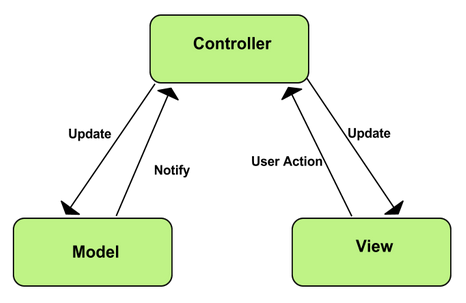
\includegraphics[height=6cm, width=9cm]{img/mvc.png}
\end{center}

SpringMVC has it's own slightly altered version of this. It works off the same principals just with a more indept controller.

\begin{center}    
	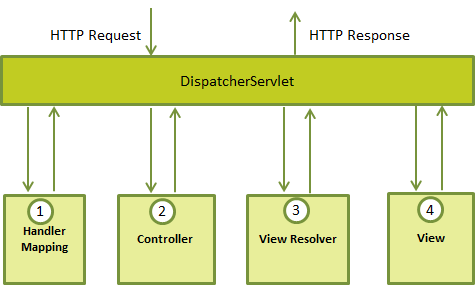
\includegraphics[height=6cm, width=10cm]{img/springmvc.png}
\end{center}

\noindent After receiving an HTTP request, DispatcherServlet consults the HandlerMapping to call the appropriate Controller. \newline

\noindent The Controller takes the request and calls the appropriate service methods based on used GET or POST method. The service method will set model data based on defined business logic and returns view name to the DispatcherServlet. \newline

\noindent The DispatcherServlet will take help from ViewResolver to pickup the defined view for the request. \newline 

\noindent Once the view is finalized, The DispatcherServlet passes the model data to the view which is finally rendered on the browser. \newline

\noindent It was very important to the project to understand this MVC concept.

\section{Hibernate ORM}

Hibernate ORM is referred usually too as Hibernate for short. Hibernate is an Object Relational Mapping framework which is what ORM stands for. ORM is a technique for mapping objects, in our case, mapping instances of Java classes and relating them to tables and columns in our chosen database. There instances of Java classes are known as POJO's or plain ordinary Java objects. Mapping of the objects to columns and tables in Hibernate is done through XML files or more recently through annotations. Hibernate XML files can be generated through Eclipse but if column names differ from field names you will find yourself spending a lot of time manually editing these files. This leads a lot of margin for error and leads to a lot of overhead. E.g Manually assigning primary keys, fields and making sure relations are properly defined. 
\noindent \newline \newline Below is an example of this 

\begin{center}    
	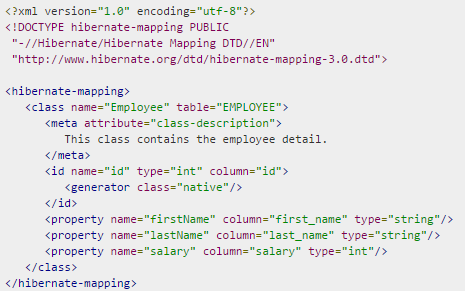
\includegraphics[height=9cm, width=14cm]{img/hibernatemapping.png}
\end{center}

Annotations, which were brought in by newer versions of Hibernate scraps the ideas of these XML files and makes things alot easier. Instead of mapping out every member variable for a class you can set up mapping now with a few simple annotations

\begin{center}    
	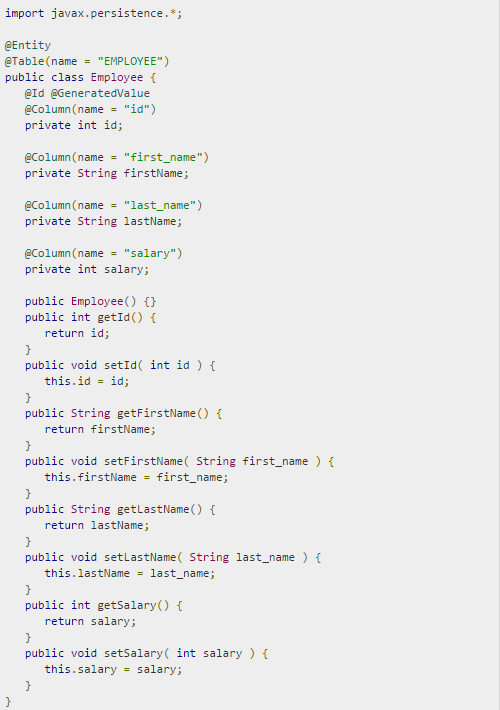
\includegraphics[height=18cm, width=12cm]{img/hibernateclass.png}
\end{center}

Hibernate also has a configuration file which must be set up. This holds connection information for the database and other settings.

\begin{center}    
	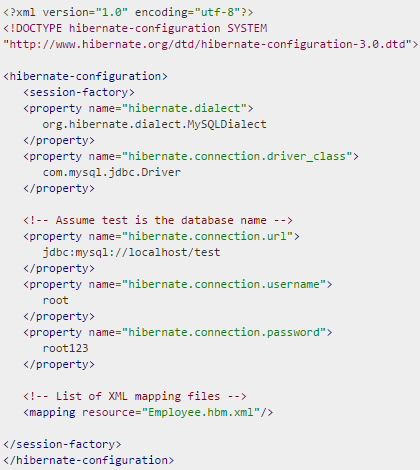
\includegraphics[height=14cm, width=13cm]{img/hibernatesettings.png}
\end{center}

Originally experimenting and learning was done using version 3 of Hibernate and used Hibernates Object Relational Mapping using XML files. These files are in typical XML format. To use this method of mapping must define the mapped files in the hibernate configuration file, if not when you try to commit the object to the database an exception is thrown. Furthermore any errors in the XML or mistypes in the mapping will stop any operations using this object.

We were successful with implementing some basic CRUD methods (Create,Read,Update and Delete). This required alot of manual configuration with the XML files. The Eclipse IDE which we used allows you to generate these hbm.xml files but they were not always correct. You must take into account that when generating these xml mapping files Eclipse has no knowledge of the database. If for whatever reason you have configured your column names in the database differently you will have configure them manually for every POJO with mapping in your project. Due to this it was best to keep field names in the POJO classes the same in both the project and the database. Hibernate will also try to generate keys and guess which field is key in the POJO or not even find the key at all. Usually the autogeneration just looked for a field called "id". Due to this you'll have to manually configure the id and it's relationship. Another major overhead of autogenerating these files is having to generate a mapping file for each class dependant on the current class you are generating the mapping for. The more relations an object has, the more files you have to configure and this was very tedious. The margin for error was high, autogeneration lead to mistakes and overall it was very rigid. This lead to very slow workflow because the IDE wouldn't return the location of errors in these files and would leave you guessing alot of the time. This experience stood to us as we now knew how to commit the objects to the database correctly. Once we had information going into the database and coming back we went back into another research phase.

Upon researching more we found alot of information about using annotations with Hibernate and that in recent version they had removed away from the traditional method of mapping using the hbm.xml files. In the case where future changes might be made to the work we have worked on it was best to research annotations more as it seemed it could speed up development and remove the need for those mapping files. We moved up a version of Hibernate and discovered Hibernate JPA Annotations. While we succeeded in getting this XML mapping working Hibernate Annotations drastically changed the workflow. Annotations removed the need for hbm.xml files and you could simply add simple annotations to the POJO class.

Creating the actual database from these classes had to be done manually. Hibernate does have the capacity to do this automatically based off the current classes but this lead to issues. The particular component was "hibernate.hbm2ddl.auto" this is called in the spring.xml file which serves as configuration file for server connection strings and to name the annotated or mapped classes. The reason this wasn't used was because it would force the generation of tables for classes we didn't use and forced the generation of tables for interfaces strangely. Some of these tables weren't needed so the tables that Hibernate generated for us were used as a guide more than anything. Using Hibernate we also found that Hibernate would look for those interface tables, this really complicated things, we only required a minimal amount of tables in the database. Due to this the decision was taken to ignore some of the composition with the POJO's and manage them manually. So in our case the class DefaultOrientationService held a set of Reviews in a ReviewSet. It was much cleaner to assign a review set id to a review and store the reviews individually that way. This solution removed the need for all these interval tables in the database. The idea was to keep our footprint on the database as light as possible. In the end we reduced the amount of tables needed in the database down too four relatively simple tables.

\section{HTML and CSS, Javascript/jQuery}

We didn't use much HTML and CSS because the sidebars and navigation bars around the content would later be updated to the style created by RoamPA's team. A simple Bootstrap was used as a template and was later removed. All of the functionality of the map was achieved using Google Maps Places API. This was all done through Javascript. Anything that needed to be done by the backend was sent through to the proper MVC routes on the server controller by using Javascript.

\chapter{System Design}


\chapter{System Evaluation}
As many pages as needed.
\begin{itemize}
\item Prove that your software is robust. How? Testing etc. 
\item Use performance benchmarks (space and time) if algorithmic.
\item Measure the outcomes / outputs of your system / software against the objectives from the Introduction.
\item Highlight any limitations or opportuni-ties in your approach or technologies used.
\end{itemize}

\chapter{Conclusion}
About three pages.

\begin{itemize}
\item Briefly summarise your context and ob-jectives (a few lines).
\item Highlight your findings from the evalua-tion section / chapter and any opportuni-ties identified.
\end{itemize}

\begin{thebibliography}{1}
	\bibitem[1]{Link1}https://www.enterprise-ireland.com/en/
	\bibitem[2]{Link2}https://www.tripadvisor.ie/
	\bibitem[3]{Link3} X
	\bibitem[4]{Link4} X
	\bibitem[5]{Link5} X
\end{thebibliography}


%= - 1 Apache Tomcat ~ http://tomcat.apache.org/ 
%= - 2 Hibernate ORM~ http://hibernate.org/
%= - 3 Spring MVC ~ https://spring.io/
%= - 4 JSP Pages ~ https://docs.oracle.com/javaee/5/tutorial/doc/bnagy.html
%= - 5 ModelViewController Explained ~ http://blog.codinghorror.com/understanding-model-view-controller/ 
%= - 6 SpringMVC ~ http://www.tutorialspoint.com/spring/spring_web_mvc_framework.htm
%= - 7 Hibernate Example ~ http://www.tutorialspoint.com/hibernate/hibernate_mapping_files.htm
%=  http://puu.sh/og17d/1dde409ae4.png
%= - 8 Hibernate Annotations ~ http://www.tutorialspoint.com/hibernate/hibernate_annotations.htm
%= - 9 Hibernate Configuration ~ http://www.tutorialspoint.com/hibernate/hibernate_configuration.htm
%= - 10 OpenStreetMap ~ http://wiki.openstreetmap.org/wiki/API
%= - 11 Leaflet ~ http://leafletjs.com/
%= - 12 Bing Maps ~ https://www.microsoft.com/maps/choose-your-bing-maps-API.aspx
%= - 13 Example Google Places ~ https://developers.google.com/places/javascript/
%= - 14 Hibernate JPA Annotations ~ https://docs.jboss.org/hibernate/stable/annotations/reference/en/html_single/
%= - API definition https://en.wikipedia.org/wiki/Application_programming_interface
%= - IDE definition http://searchsoftwarequality.techtarget.com/definition/integrated-development-environment
%= - Eclipse https://eclipse.org/